\documentclass[a4paper]{article}
\usepackage[top=1in, bottom=1.25in, left=1.25in, right=1.25in]{geometry}
\usepackage{amsmath}
\usepackage{multicol}
\usepackage{graphicx}
\usepackage[utf8]{inputenc}
\usepackage[english]{babel}
\setlength{\parskip}{0.03cm plus4mm minus3mm}
\RequirePackage{ltxcmds}[2010/12/07]
\usepackage{array}
\usepackage{hyperref}
\renewcommand{\arraystretch}{1.5}
%\setlength{\arrayrulewidth}{1mm}
%opening
\title{MQAM transmitter}

\begin{document}

\maketitle
This block generates one or two optical signals. A schematic representation of this block is shown in figure \ref{MQAM_transmitter_block_diagram}.

\begin{figure}
	\centering
	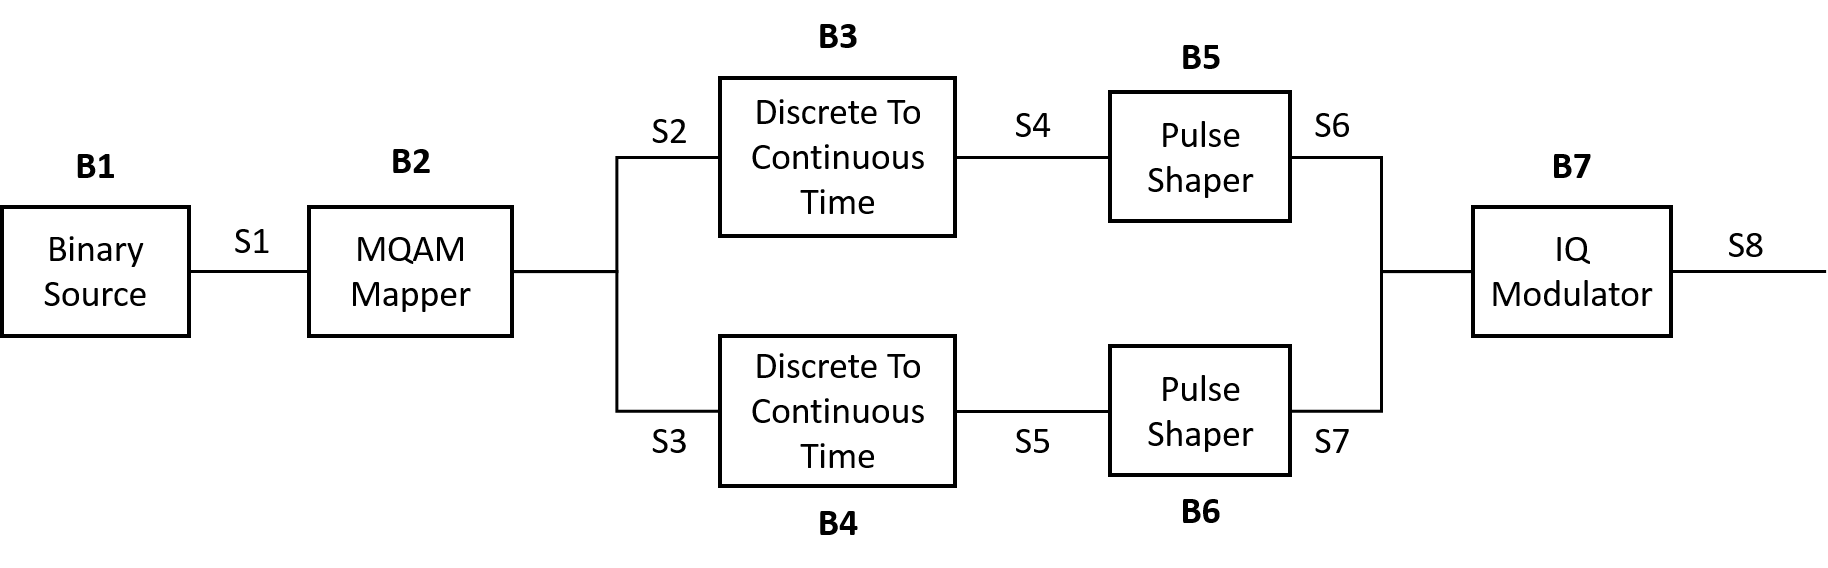
\includegraphics[width=\textwidth]{MQAM_transmitter_block_diagram}
	\caption{Schematic representation of the block MQAM transmitter.}\label{MQAM_transmitter_block_diagram}
\end{figure}

\subsection*{Input parameters}

This block has a special set of functions that allow the user to change the basic configuration of the transmitter. The list of input parameters, functions used to change them and the values that each one can take are summarized in table \ref{table}.

\begin{table}
\begin{center}
	\begin{tabular}{| m{5cm} | m{5,5cm} | m{5cm} | }
		\hline 
		\textbf{Input parameters} & \textbf{Function} & \textbf{Accepted values} \\ \hline
		Mode & setMode() & PseudoRandom \newline Random \newline DeterministicAppendZeros \newline DeterministicCyclic \\ \hline
		Bit period & setBitPeriod() & double \\ \hline
		Pattern length & setPatternLength() & int \\ \hline
		Number of bits & setNumberOfBits() & long \\ \hline
		Number of samples per symbol & setNumberOfSamplesPerSymbol() & int \\ \hline
		Roll of factor & setRollOfFactor() & double $\in$ [0,1] \\ \hline
		IQ amplitudes & setIqAmplitudes() & Vector of coordinate points in the I-Q plane \newline \textbf{Example} for a 4-qam mapping: \{ \{ 1.0, 1.0 \}, \{ -1.0, 1.0 \}, \{ -1.0, -1.0 \}, \{ 1.0, -1.0 \} \} \\ \hline
		Output optical power & setOutputOpticalPower() & int \\ \hline
		Save internal signals & setSaveInternalSignals() & True/False \\
		\hline
	\end{tabular}
	\caption{List of input parameters of the block MQAM transmitter} \label{table} 
\end{center}
\end{table}

%\begin{itemize}
%	\item setMode(PseudoRandom);
%	\item setBitPeriod(1.0/50e9);
%	\linebreak (double)
%	\item setPatternLength(3);
%	\linebreak (int)
%	\item setNumberOfBits(10000);
%	\linebreak (long)
%	\item setNumberOfSamplesPerSymbol(32);
%	\linebreak (int)
%	\item setRollOffFactor(0.9);
%	\linebreak (double $\in$ [0,1])
%	\item setIqAmplitudes(\{ \{ 1, 1 \}, \{ -1, 1 \}, \{ -1, -1 \}, \{ 1, -1 \} \});
%	\item setOutputOpticalPower\_dBm(0);
%	\item setSaveInternalSignals(true);
%\end{itemize}


\subsection*{Methods}

MQamTransmitter(vector$<$Signal *$>$ \&inputSignal, vector$<$Signal *$>$ \&outputSignal);
\bigbreak

void set(int opt);
\bigbreak
void setMode(BinarySourceMode m) \{ B1.setMode(m); \};
\bigbreak
BinarySourceMode const getMode(void) \{ return B1.getMode(); \};
\bigbreak
void setProbabilityOfZero(double pZero) \{ B1.setProbabilityOfZero(pZero); \};
\bigbreak
double const getProbabilityOfZero(void) \{ return B1.getProbabilityOfZero(); \};
\bigbreak
void setBitStream(string bStream) \{ B1.setBitStream(bStream); \};
\bigbreak
string const getBitStream(void) \{ return B1.getBitStream(); \};
\bigbreak
void setNumberOfBits(long int nOfBits) \{ B1.setNumberOfBits(nOfBits); \}
\bigbreak
long int const getNumberOfBits(void) \{ return B1.getNumberOfBits();  \}
\bigbreak
void setPatternLength(int pLength) \{ B1.setPatternLength(pLength); \}
\bigbreak
int const getPatternLength(void) \{ return B1.getPatternLength(); \}
\bigbreak
void setBitPeriod(double bPeriod) \{B1.setBitPeriod(bPeriod);\};
double const getBitPeriod(void) \{ return B1.getBitPeriod(); \}
\bigbreak
void setM(int mValue)\{B2.m = mValue;\};
int const getM(void) \{ return B2.m; \};
\bigbreak
%void setIqAmplitudes(vector$<$t$_$iqValues$>$ iqAmplitudesValues) \{ B2.m = iqAmplitudesValues.size(); B2.iqAmplitudes.resize(B2.m);B2.iqAmplitudes = iqAmplitudesValues; \};
\bigbreak
%vector$<$t$_$iqValues$>$ const getIqAmplitudes(void) \{ return B2.iqAmplitudes; \};
\bigbreak
void setNumberOfSamplesPerSymbol(int n)\{ B3.setNumberOfSamplesPerSymbol(n); B4.setNumberOfSamplesPerSymbol(n); \};
\bigbreak
int const getNumberOfSamplesPerSymbol(void)\{ return B3.getNumberOfSamplesPerSymbol(); \};
\bigbreak
void setRollOffFactor(double rOffFactor)\{ B5.setRollOffFactor(rOffFactor); B6.setRollOffFactor(rOffFactor); \};
\bigbreak
double const getRollOffFactor(void)\{ return B5.getRollOffFactor(); \};
\bigbreak
void setSeeBeginningOfImpulseResponse(bool sBeginningOfImpulseResponse)\{ B5.setSeeBeginningOfImpulseResponse(sBeginningOfImpulseResponse); B6.setSeeBeginningOfImpulseResponse(sBeginningOfImpulseResponse); \};
\bigbreak
double const getSeeBeginningOfImpulseResponse(void)\{ return B5.getSeeBeginningOfImpulseResponse(); \};
\bigbreak
%void setOutputOpticalPower(t$_$real outOpticalPower) \{ B7.outputOpticalPower = outOpticalPower; \};
\bigbreak
%t$_$real const getOutputOpticalPower(void) \{ return B7.outputOpticalPower; \};
\bigbreak
%void setOutputOpticalPower$_$dBm(t$_$real outOpticalPower$_$dBm) \{ B7.outputOpticalPower = 1e-3*pow(10, outOpticalPower$_$dBm / 10); \};
\bigbreak
%t$_$real const getOutputOpticalPower$_$dBm(void) \{ return 10*log10(B7.outputOpticalPower/1e-3); \}

\subsection*{Functional description}

This block generates an optical signal (output signal 1 in figure \ref{MQAM_transmitter_block_diagram}). The binary signal generated in the internal block Binary Source (block B1 in figure \ref{MQAM_transmitter_block_diagram}) can be used to perform a Bit Error Rate (BER) measurement and in that sense it works as an extra output signal (output signal 2 in figure \ref{MQAM_transmitter_block_diagram}). 

\subsection*{Output Signals}

\subparagraph*{Number:} 1 or 2 optical and 1 binary

\subparagraph*{Type:} Optical signal

\subsection*{Example} 

\subsection*{Sugestions for future improvement}


\end{document}